%%==================================================
%% ch3.tex for BIT Master Thesis
%% modified by yang yating
%% version: 0.2
%% last update: Feb 16th, 2017
%%==================================================


% \bibliographystyle{bit2} %[此处用于每章都生产参考文献]
\chapter{公式、图像和表格}
\label{chap:example}
公式、图表和插图广泛使用于学位论文中,并且在正文内存在较多的交叉引用,对他们的高效处理也是\LaTeX{}的优势之一。公式、图表和插图在定义时的共同特点包含:定义中需要设定引用标签、设置图表名称。定义时,图表摆放位置并无要求,\LaTeX{}会根据文稿内容自动计算图表摆放位置,不会出现表格窜行的问题。

\section{公式与数学环境}
\label{sec:eqn}

\subsection{公式及术语表}
\label{sec:eqn}

公式定义的内容包含在\verb|\begin{equation}|\verb|\end{equation}|之间。为方便,公式的编辑可以采用在线的\LaTeX{}公式编辑器。公式的编号格式可以在.sty文件夹下的格式文件中定义,公式中涉及的术语表也需要在公式后面进行对应标记。一般的\LaTeX{}编辑器如Winedit、texmaker等都有公式编辑器。

{\bf{实例1:}} 以下是L-B非稳态流动升力模型,公式引用为公式\ref{eqn:LBmodel}。该公式的术语列表见 表 \ref{tab:LB-parameters}。
\begin{equation}
 \label{eqn:LBmodel}
   C_{L}=C_{L0}+C_{L\alpha }\left ( \frac{1+\sqrt{X}}{2} \right )\alpha 
\end{equation}

\begin{lstlisting}[language={[LaTeX]TeX}, caption={L-B非稳态流动升力模型}]
\begin{equation}
 \label{eqn:LBmodel}
   C_{L}=C_{L0}+C_{L\alpha }\left ( \frac{1+\sqrt{X}}{2} \right )\alpha 
\end{equation}
\end{lstlisting}

\subsection{长公式排版}


《Math mode》里有举一个长公式排版的例子如下。《Math mode》有十分丰富实用的例子,感兴趣的同学可以参考一下。

\begin {multline}
  \frac {1}{2}\Delta (f_{ij}f^{ij})=
  2\left (\sum _{i<j}\chi _{ij}(\sigma _{i}-
    \sigma _{j}) ^{2}+ f^{ij}\nabla _{j}\nabla _{i}(\Delta f)+\right .\\
  \left .+\nabla _{k}f_{ij}\nabla ^{k}f^{ij}+
    f^{ij}f^{k}\left [2\nabla _{i}R_{jk}-
      \nabla _{k}R_{ij}\right ]\vphantom {\sum _{i<j}}\right )
\end{multline}

\begin{lstlisting}[language={[LaTeX]TeX}, caption={长公式排版}]
\begin {multline}
  \frac {1}{2}\Delta(f_{ij}f^{ij})=
  2\left(\sum_{i<j}\chi_{ij}(\sigma_{i}-
    \sigma_{j}) ^{2}+ f^{ij}\nabla_{j}\nabla_{i}(\Delta f)+\right.\\
  \left.+\nabla_{k}f_{ij}\nabla ^{k}f^{ij}+
    f^{ij}f^{k}\left [2\nabla_{i}R_{jk}-
      \nabla_{k}R_{ij}\right]\vphantom{\sum_{i<j}}\right )
\end{multline}
\end{lstlisting}

\subsection{定理环境}

在~bitmaster-xetex.cfg~中定义了丰富的定理环境
algo(算法),thm(定理),lem(引理),prop(命题),cor(推论),defn(定义),conj(猜想),exmp(例),rem(注),case(情形),
bthm(断言定理),blem(断言引理),bprop(断言命题),bcor(断言推论)。
amsmath还提供了一个proof(证明)的环境。
这里举一个``定理''和``证明''的例子。
\begin{thm}[留数定理]
\label{thm:res}
  假设$U$是复平面上的一个单连通开子集,$a_1,\ldots,a_n$是复平面上有限个点,$f$是定义在$U\backslash \{a_1,\ldots,a_n\}$上的全纯函数,
  如果$\gamma$是一条把$a_1,\ldots,a_n$包围起来的可求长曲线,但不经过任何一个$a_k$,并且其起点与终点重合,那么:

  \begin{equation}
    \label{eq:res}
    \ointop_{\gamma}f(z)\,\mathrm{d}z = 2\uppi\mathbf{i}\sum^n_{k=1}\mathrm{I}(\gamma,a_k)\mathrm{Res}(f,a_k)
  \end{equation}

  如果$\gamma$是若尔当曲线,那么$\mathrm{I}(\gamma, a_k)=1$,因此:

  \begin{equation}
    \label{eq:resthm}
    \ointop_{\gamma}f(z)\,\mathrm{d}z = 2\uppi\mathbf{i}\sum^n_{k=1}\mathrm{Res}(f,a_k)
  \end{equation}

      % \oint_\gamma f(z)\, dz = 2\pi i \sum_{k=1}^n \mathrm{Res}(f, a_k ). 

  在这里,$\mathrm{Res}(f, a_k)$表示$f$在点$a_k$的留数,$\mathrm{I}(\gamma,a_k)$表示$\gamma$关于点$a_k$的卷绕数。
  卷绕数是一个整数,它描述了曲线$\gamma$绕过点$a_k$的次数。如果$\gamma$依逆时针方向绕着$a_k$移动,卷绕数就是一个正数,
  如果$\gamma$根本不绕过$a_k$,卷绕数就是零。

  定理\ref{thm:res}的证明。
  
  \begin{proof}
    首先,由……

    其次,……

    所以……
  \end{proof}
  
\end{thm}

上面的公式例子中,有一些细节需要注意。微分号d应该使用``直立体'',也就是用mathrm包围起来。
并且,微分号和被积函数之间应该有一段小间隔,可以插入\verb+\,+得到。
斜体的$d$通常只作为一般变量。
i,j作为虚数单位时,也应该使用``直立体'',为了明显,还加上了粗体,例如\verb+\mathbf{i}+。斜体$i,j$通常用作表示``序号''。
其他字母在表示常量时,也推荐使用``直立体'',譬如,圆周率$\uppi$(需要upgreek宏包),自然对数的底$\mathrm{e}$。


\section{向文档中插入图像}
\label{sec:insertimage}

\subsection{支持的图片格式}
\label{sec:imageformat}

\XeTeX~ 可以很方便地插入~PDF、EPS、PNG、JPG~格式的图片。

在学位论文中,插图地使用简单地分为两类:单列图片和多列图片。图片地格式包含*.jpg、*.eps、*.pdf,既可以是位图也可以是矢量图,在插入图片是可以定义其高度和宽度。

插入PNG/JPG的例子如\ref{fig:png-jpg}所示。
这两个水平并列放置的图共享一个``图标题''(table caption),没有各自的小标题。

\begin{figure}[!htp]
  \centering
  
\includegraphics[width=0.35\textwidth]{figures/BIT}
  \hspace{1cm}
  
\includegraphics[width=0.35\textwidth]{figures/BIT-CS}
  \caption{校徽以及计算机学院LOGO}
  \label{fig:png-jpg}
\end{figure}

\begin{lstlisting}[language={[LaTeX]TeX}, caption={插入PNG/JPG}]
\begin{figure}[!htp]
  \centering
  
\includegraphics[width=0.3\textwidth]{figures/BIT}
  \hspace{1cm}
  
\includegraphics[width=0.3\textwidth]{figures/BIT-CS}
  \caption{校徽以及计算机学院LOGO}
  \label{fig:png-jpg}
\end{figure}
\end{lstlisting}

这里还有插入eps图像和pdf图像的例子,如图\ref{fig:pdfeps}。这里将EPS和PDF图片作为子图插入,每个子图有自己的小标题。并列子图的功能是使用~subfigure~宏包提供的。

\begin{figure}[!b]
  \centering
  \subfigure[EPS Figure]{
    \label{fig:epspdf:a} %% label for first subfigure
    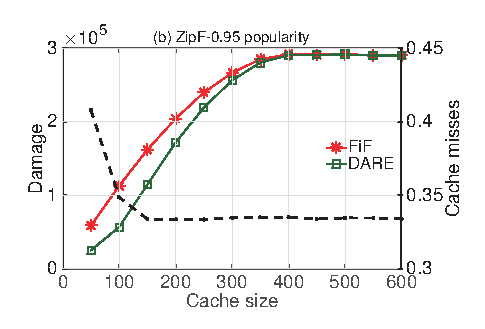
\includegraphics[width=0.45\textwidth]{figures/pic-eps}}
  \subfigure[PDF Figure]{
    \label{fig:epspdf:b} %% label for second subfigure
    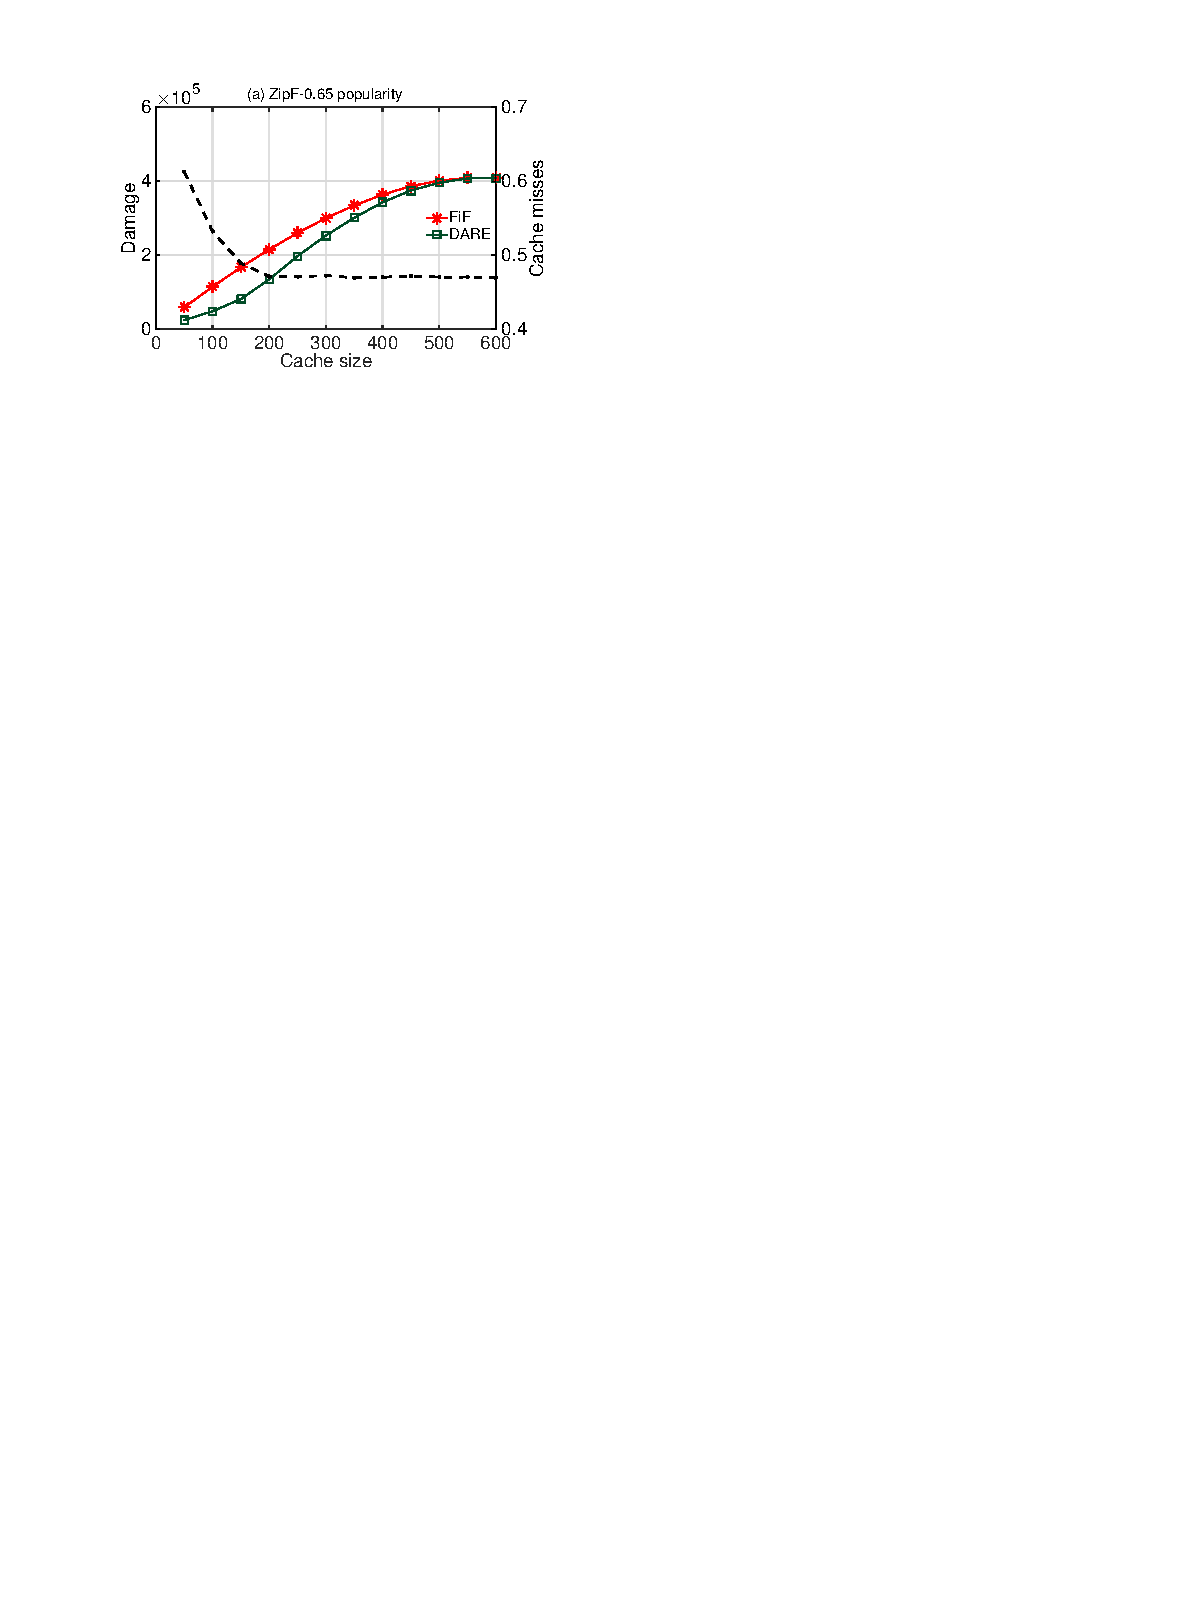
\includegraphics[width=0.45\textwidth]{figures/pic-pdf.pdf}}
  \caption{插入eps图像和pdf图像}
  \label{fig:pdfeps}
\end{figure}

\begin{lstlisting}[language={[LaTeX]TeX}, caption={插入eps图像和pdf图像}][!htp]
\begin{figure}
  \centering
  \subfigure[EPS Figure]{
    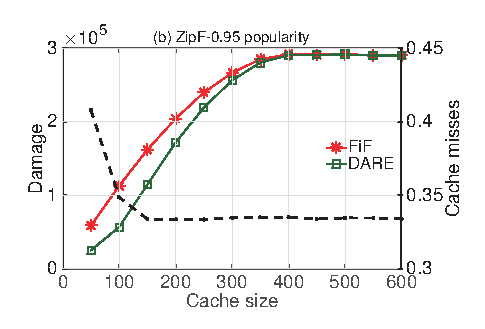
\includegraphics[width=0.45\textwidth]{figures/pic-eps}}
  \subfigure[PDF Figure]{
    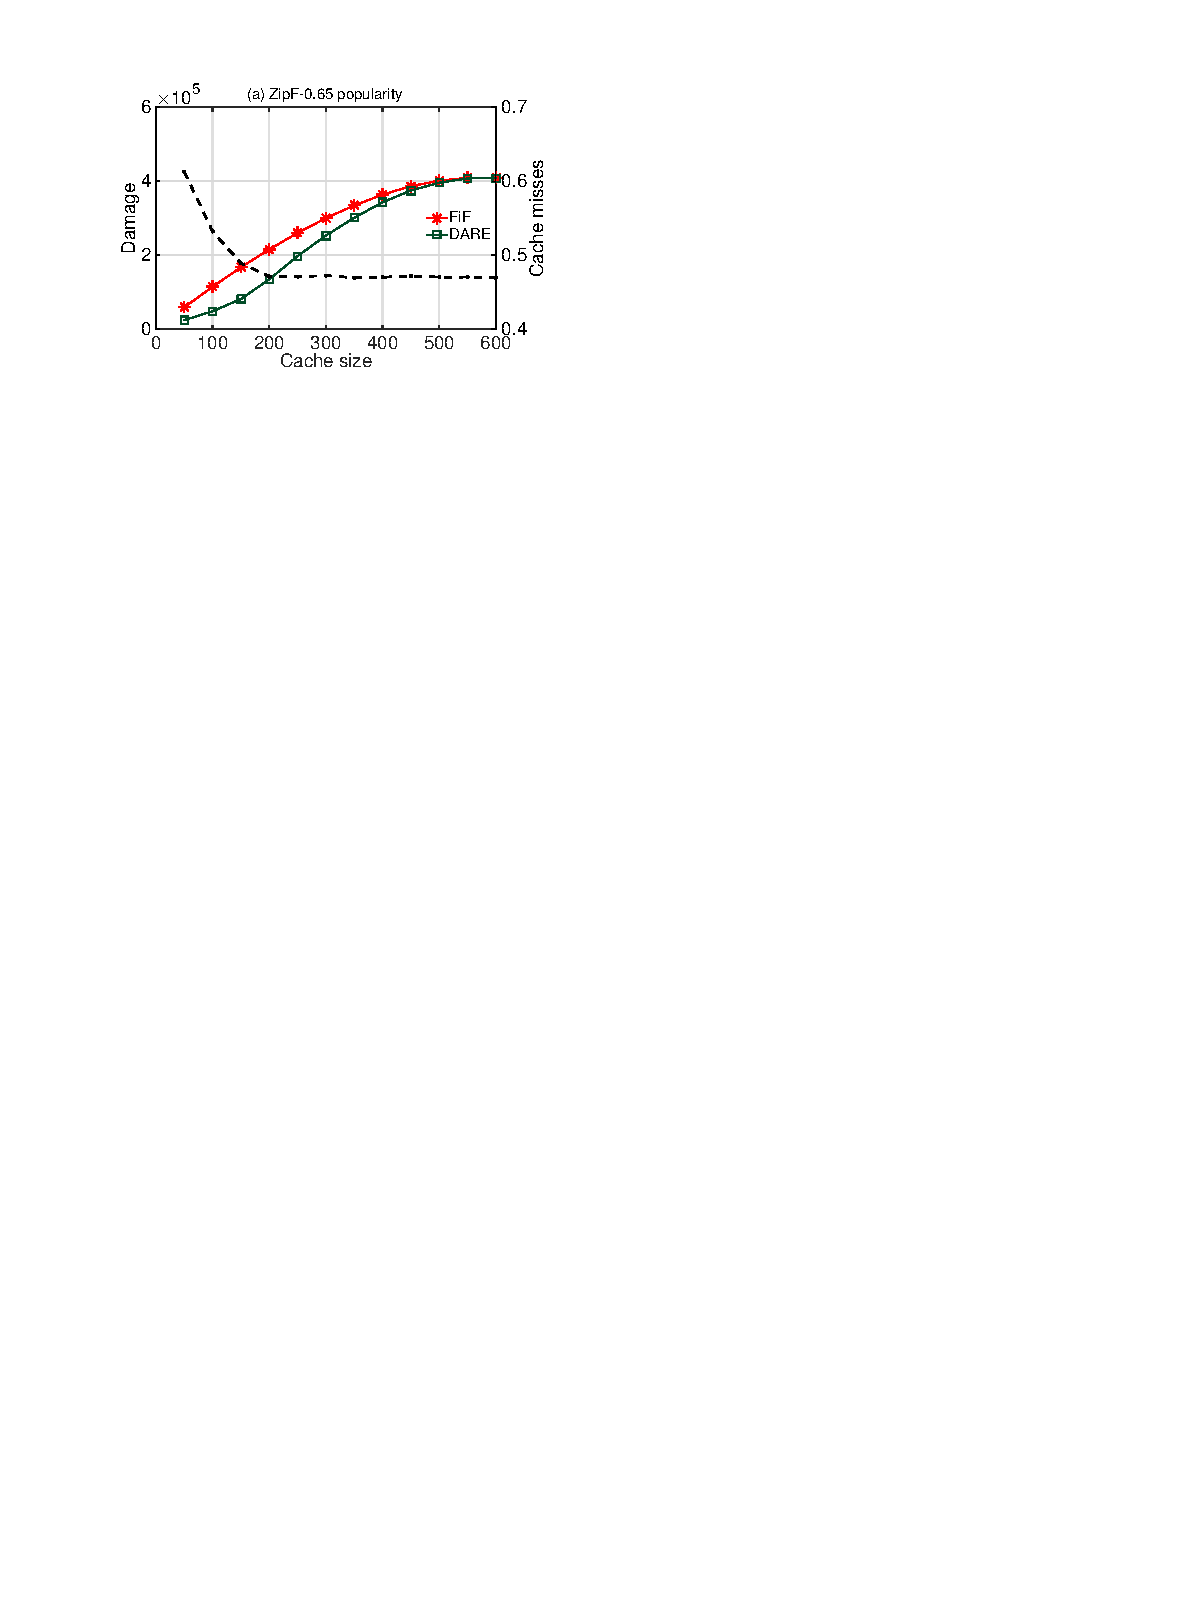
\includegraphics[width=0.45\textwidth]{figures/pic-pdf.pdf}}
  \caption{插入eps图像和pdf图像}
\end{figure}
\end{lstlisting}

更多关于~\LaTeX~ 插图的例子可以参考《~\LaTeX~插图指南》。

\subsection{长标题的换行}
\label{sec:longcaption}

图\ref{fig:longcaptionbad}和图\ref{fig:longcaptiongood}都有比较长图标题,通过对比发现,图\ref{fig:longcaptiongood}的换行效果更好一些。
其中使用了minipage环境来限制整个浮动题的宽度。

\begin{figure}[!htp]
 \centering
 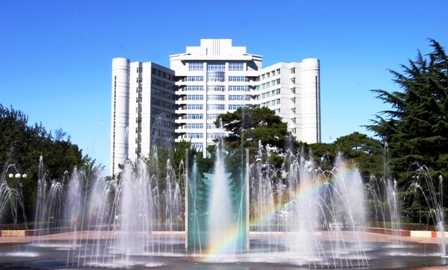
\includegraphics[width=10cm]{figures/pic1}
 \caption{BIT是我国历史最悠久的高等学府之一,是教育部直属、工信部共建的全国重点大学,985,211}
 \label{fig:longcaptionbad}
\end{figure}

\begin{figure}[!hbp]
  \centering
  \begin{minipage}[b]{0.6\textwidth}
  \captionstyle{\centering}
  \centering
  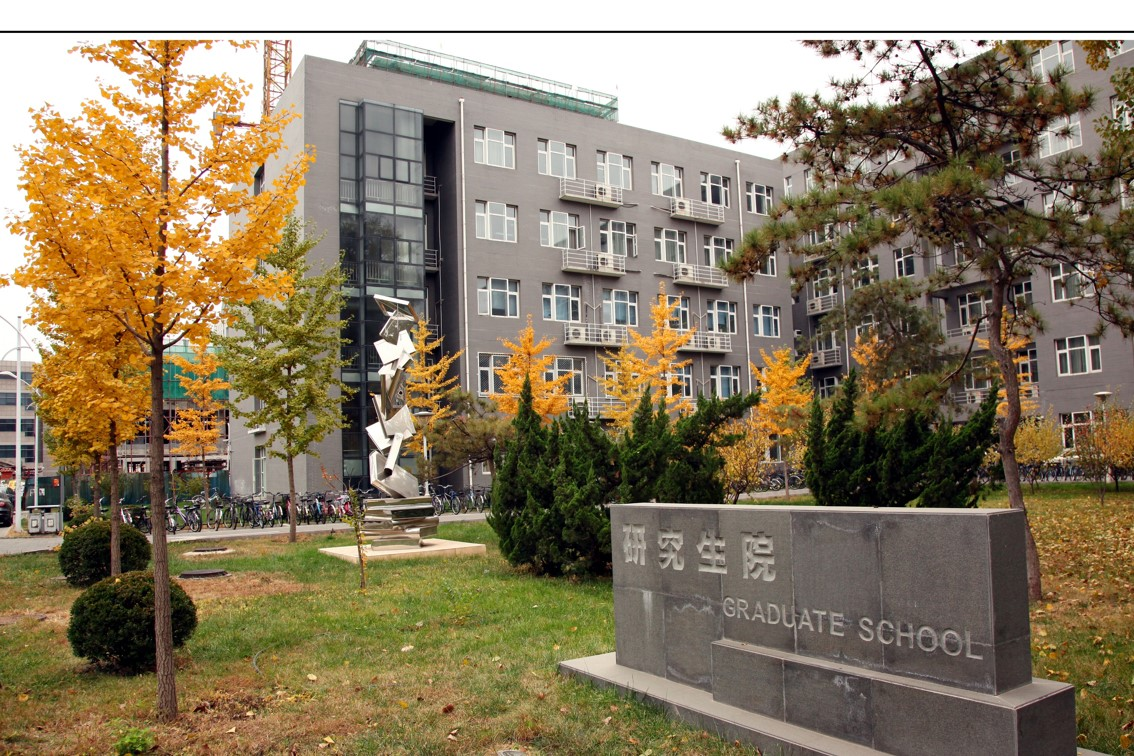
\includegraphics[width=10cm]{figures/pic2}
  \caption{BIT是我国历史最悠久的高等学府之一,是教育部直属、工信部共建的全国重点大学,985,211}
  \label{fig:longcaptiongood}
   \end{minipage}     
\end{figure}

\begin{lstlisting}[language={[LaTeX]TeX}, caption={长标题的换行}]
\begin{figure}[!htp]
 \centering
 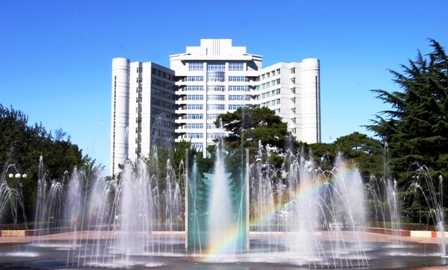
\includegraphics[width=10cm]{figures/pic1}
 \caption{BIT是我国历史最悠久的高等学府之一,是教育部直属、工信部共建的全国重点大学,985,211}
 \label{fig:longcaptionbad}
\end{figure}

\begin{figure}[!hbp]
  \centering
  \begin{minipage}[b]{0.6\textwidth}
  \captionstyle{\centering}
  \centering
  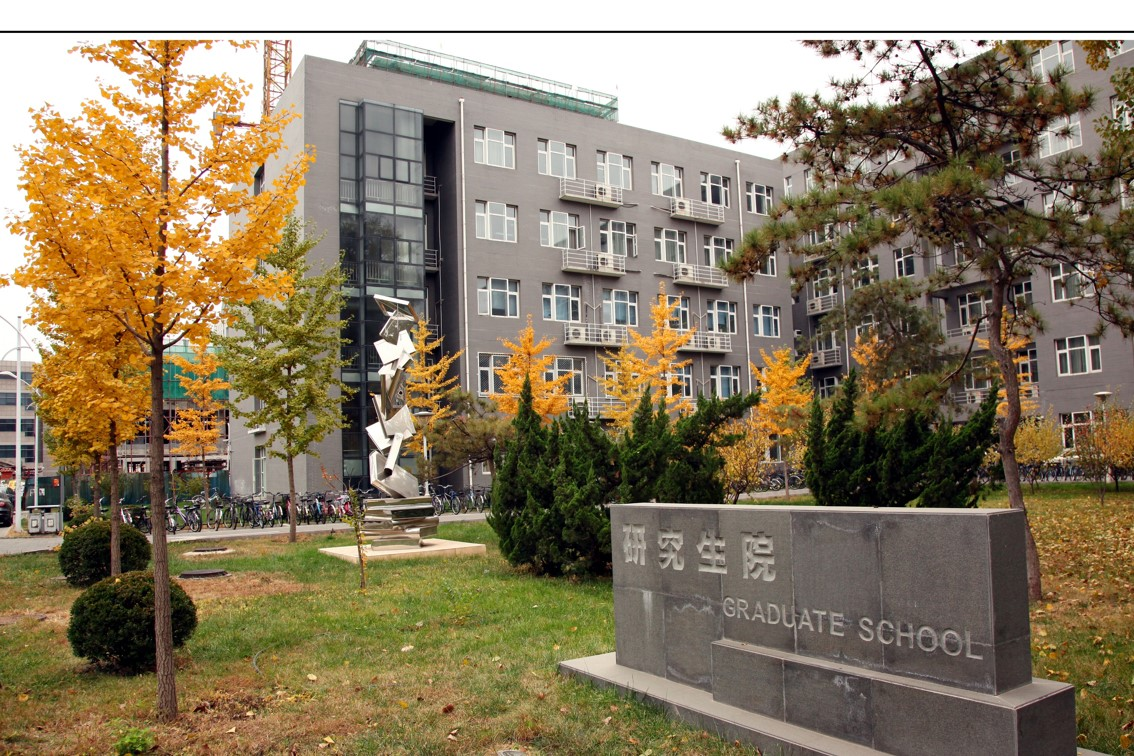
\includegraphics[width=10cm]{figures/pic2}
  \caption{BIT是我国历史最悠久的高等学府之一,是教育部直属、工信部共建的全国重点大学,985,211}
  \label{fig:longcaptiongood}
   \end{minipage}     
\end{figure}
\end{lstlisting}
  
\section{表格的例子}
\label{sec:tab}

表格的定义和引用已经在第~\ref{sec:refofFigAndTab}节中介绍,表格内容包含在\textbackslash begin\{table\}和\textbackslash end\{table\}之间。这里给出一些表格的例子。

\begin{table}[htb]               % no placement specified: defaults to here, top, bottom, page
\centering
 \begin{center}
  \caption{L-B模型中参数的物理意义}
  \label{tab:LB-parameters}
  \begin{tabular}{cl}
      \toprule
       Parameters & Physical meaning       \\
      \midrule   % \hline
       $C_{L\alpha}$ & Lift curve slope \\
       $a_{1}$ & Controls the shape of the stall curve \\
       $\alpha^{\star}$ & The break point at which $X=0.5$ \\
       $\tau_{1}$ & Represents the tendency of the model to track the static curve \\
       $\tau_{2}$ & Gives the model lift overshoot \\
      \bottomrule
  \end{tabular}
 \end{center}
\end{table}

\begin{lstlisting}[language={[LaTeX]TeX}, caption={插入表格}]
\begin{table}[htb]
\centering
 \begin{center}
  \caption{L-B模型中参数的物理意义}
  \begin{tabular}{cl}
      \toprule
       Parameters & Physical meaning       \\
      \midrule 
       $C_{L\alpha}$ & Lift curve slope \\
       $a_{1}$ & Controls the shape of the stall curve \\
       $\alpha^{\star}$ & The break point at which $X=0.5$ \\
       $\tau_{1}$ & Represents the tendency of the model to track the static curve \\
       $\tau_{2}$ & Gives the model lift overshoot \\
      \bottomrule
  \end{tabular}
 \end{center}
\end{table}
\end{lstlisting}

再给出一些表格的例子,如表\ref{tab:firstone}所示。

\begin{table}[!htp]
  \centering
  \bicaption[tab:firstone]{指向一个表格的表目录索引}{一个颇为标准的三线表格\footnotemark[1]}{Table}{A Table}
  \begin{tabular}{@{}llr@{}} \toprule
    \multicolumn{2}{c}{Item} \\ \cmidrule(r){1-2}
    Animal & Description & Price (\$)\\ \midrule
    Gnat & per gram & 13.65 \\
    & each & 0.01 \\
    Gnu & stuffed & 92.50 \\
    Emu & stuffed & 33.33 \\
    Armadillo & frozen & 8.99 \\ \bottomrule
  \end{tabular}
\end{table}

下面一个是一个更复杂的表格,用threeparttable实现带有脚注的表格,如表\ref{tab:footnote}。

\begin{table}[!htp]
  \bicaption[tab:footnote]{出现在表目录的标题}{一个带有脚注的表格的例子}{Table}{A Table with footnotes}
  \centering
  \begin{threeparttable}[b]
     \begin{tabular}{ccd{4}cccc}
      \toprule
      \multirow{2}{6mm}{total}&\multicolumn{2}{c}{20\tnote{1}} & \multicolumn{2}{c}{40} &  \multicolumn{2}{c}{60}\\
      \cmidrule(lr){2-3}\cmidrule(lr){4-5}\cmidrule(lr){6-7}
      &www & k & www & k & www & k \\
      \midrule
      &$\underset{(2.12)}{4.22}$ & 120.0140\tnote{2} & 333.15 & 0.0411 & 444.99 & 0.1387 \\
      &168.6123 & 10.86 & 255.37 & 0.0353 & 376.14 & 0.1058 \\
      &6.761    & 0.007 & 235.37 & 0.0267 & 348.66 & 0.1010 \\
      \bottomrule
    \end{tabular}
    \begin{tablenotes}
    \item [1] the first note.% or \item [a]
    \item [2] the second note.% or \item [b]
    \end{tablenotes}
  \end{threeparttable}
\end{table}



\section{参考文献管理}
\label{sec:reference}
\subsection{将参考文献的内容与表现分离}

BIT-Thesis论文模板使用BibTeX处理参考文献,
BibTeX是最为流行的参考文献数据组织格式之一。它的出现让我们摆脱手写参考文献条目
的麻烦。
当然,使用者也可以手动编参考文献item,直接插入文档中。但是,有BibTeX帮助,处理起参考文献更为简单。我们还可以通过参考文献格式的支持,让同一份BibTeX数据库生成不同格式的参考文
献列表。

参考文献的具体内容就是reference文件夹下的chap\textit{xx}.bib,参考文献的元数据(名称、作者、出处等)以一定的格式保存在这些纯文本文件中。
.bib文件也可以理解为参考文献的``数据库'',正文中所有引用的参考文件条目都会从这些文件中``析出''。
控制参考文献条目``表现形式''(格式)的是.bst文件。.bst文件定义了参考文献风格,使用不同的参考文献风格能将同一个参考文献条目输出成不同的格式。
当然,一个文档只能使用一个参考文献风格。
按照学校要求,本模板使用的是国标GBT7714风格的参考文献。

BibTeX的工作过程是这样的:
BibTeX读取.aux(第一次运行latex得到的)查看参考文献条目,
然后到.bib中找相关条目的信息,
最后根据.bst的格式要求将参考文献条目格式化输出,写到.bbl文件中。
在运行latex将.bbl插入文档之前,可以用文本编辑器打开它,做一些小的修改。
.bbl的格式和你自己手动写item很相似,它已经被赋予了一定的``表现形式''。

.bib数据库中的参考文献条目可以手动编写,也可以在google的学术搜索中找到。
各大数据库也支持将参考文献信息导出为.bib,省时省力。
以Google学术搜索为例:在``学术搜索设置''中,将``文献管理软件''设为``显示导入BibTeX''的连接,保存退出。
然后学术搜索找到文献下会有``导出到BibTeX''连接,点击后Firefox会打开新的标签页,出现类似代码\ref{googlescholar}所示的内容。
请注意,这个条目离``规范''还有一些距离。

  \begin{lstlisting}[caption={从Google Scholar找到的,但并不规范的.bib条目}, label=googlescholar, float, escapeinside="", numbers=none]
    @phdthesis{" 白2008信用风险传染模型和信用衍生品的定价 ",
      title={{" 信用风险传染模型和信用衍生品的定价 "}},
      author={" 白云芬 "},
      year={2008},
      school={" 上海交通大学 "}
    } 
  \end{lstlisting}

  上面的.bib条目的``名字''\cndash{}``白2008信用风险传染模型和信用衍生品的定价'',包含~ASCII~以外的字符,BibTeX无法处理;
  条目还缺少了address域,这样编译出来的结果会出现``地址不详'';
  并且,条目还缺少language域,BibTeX需要language域来判断是否是中文参考文献。
  将上面的条目修正(改英文名、增加address和language域),复制到本地的.bib文件中就可以了。
  显然,这里描述的是参考文献的内容,而不是表现形式。

  \begin{lstlisting}[caption={一个符合规范的.bib条目}, label=itemok, float, escapeinside="", numbers=none]
@article{ Jiang2005Size,
  title={ 形状记忆聚合物研究现状与发展 },
  author={ 姜敏 and 彭少贤 and 郦华兴 },
  journal={ 现代塑料加工应用 },
  volume={17},
  number={2},
  pages={53-56},
  year={2005},
}
  \end{lstlisting}

由于中英文参考文献处理起来有差异,所以需要在参考文献中标注是否是中文文献。
确切地说,BibTeX并不具有区分中英文参考文献的能力。.bib是“参考文献的内容”,而控制参考文献表现(格式)的是.bst文件,本模板附带的是GBT7714-2005NLang.bst。
GBT7714-2005NLang.bst中规定:.bib中的条目,如果条目的``language''域非空,就被认为是中文文献,否则被认为是英文文献。
例如,刚才的文献,就会被认为是中文参考文献,采取一些针对中文的处理方式。

最后,这个条目被bibtex处理后,赋予了一定的``表现形式'',在.bbl文件中以下面的样子出现。
还可以对它进行小的修改,但较为麻烦。然后再次运行latex之后,它将被插入到文档中。

\begin{lstlisting}[caption={.bbl中被格式化之后的条目}, escapeinside="", numbers=none]
\bibitem{Jiang2005Size}
	姜敏, 彭少贤, 郦华兴.
	形状记忆聚合物研究现状与发展~[J].
	现代塑料加工应用, 2005, 17~(2):  53--56.
\end{lstlisting}


\subsection{在正文中引用参考文献}

参考文献可以分章节管理,只需要在主文件中的参考文献中都包含进去就可以,如\verb+\bibliography{chap1,figures/chap2,...}+。

正文中引用参考文献时\citep{Jiang2005Size},用\verb+\upcite{key1,key2,key3...}+可以产生“上标引用的参考文献”,
如\upcite{Meta_CN,chen2007act,DPMG}。
使用\verb+\cite{key1,key2,key3...}+则可以产生水平引用的参考文献,例如\cite{JohnD,zhubajie,IEEE-1363}。
请看下面的例子,将会穿插使用水平的和上标的参考文献:关于书的\cite{Meta_CN,JohnD,IEEE-1363},关于期刊的\upcite{chen2007act,chen2007ewi},
会议论文\cite{DPMG,kocher99,cnproceed},
硕士学位论文\cite{zhubajie,metamori2004},博士学位论文\upcite{shaheshang,FistSystem01,bai2008},标准文件\cite{IEEE-1363},技术报告\upcite{NPB2},电子文献\cite{xiaoyu2001, CHRISTINE1998}。

最后总结一些注意事项:
\begin{itemize}
\item  参考文献只有在正文中被引用了,才会在最后的参考文献列表中出现;
\item  参考文献``数据库文件''.bib是纯文本文件,请使用~UTF-8~编码,不要使用~GBK~编码;
\item  参考文献条目中通过~language~域是否为空判断是否是中文文献;
\item  参考文献条目同样有“内容”和“表现形式”之分,这种可控性是BibTeX带来的。
\end{itemize}


\section{用~listings~插入源代码}

这里给使用~listings~宏包插入源代码的例子,这里是一段C代码。另外,listings宏包可以实现各种复杂、漂亮的效果,想要进一步学习的同学,可以参考《The Listings Package》。

{\color{blue}
\begin{enumerate}
\item[] ~\verb|\begin{lstlisting}[language={C}, caption={一段C源代码}]|
\item[] ~\verb|#include <stdio.h>| 
\item[] ~\verb|...|
\item[] ~\verb|\end{lstlisting}|
\end{enumerate}}


\begin{lstlisting}[language={C}, caption={一段C源代码}]
#include <stdio.h>
#include <unistd.h>
#include <sys/types.h>
#include <sys/wait.h>

int main() {
  pid_t pid;

  switch ((pid = fork())) {
  case -1:
    printf("fork failed\n");
    break;
  case 0:
    /* child calls exec */
    execl("/bin/ls", "ls", "-l", (char*)0);
    printf("execl failed\n");
    break;
  default:
    /* parent uses wait to suspend execution until child finishes */
    wait((int*)0);
    printf("is completed\n");
    break;
  }

  return 0;
}
\end{lstlisting}

再给出一个插入MATLAB代码的例子。

{\color{blue}
\begin{enumerate}
\item[] ~\verb|\begin{lstlisting}[language={matlab}, caption={一段MATLAB源代码}]|
\item[] ~\verb|function paper1| 
\item[] ~\verb|r=0.05;|
\item[] ~\verb|n=100;|
\item[] ~\verb|...|
\item[] ~\verb|\end{lstlisting}|
\end{enumerate}}

\begin{lstlisting}[language={matlab}, caption={一段MATLAB源代码}]
function paper1
r=0.05;
n=100;
T=1;
X=1;
v0=0.8;
sigma=sqrt(0.08);
deltat=T/n;
for i=1:n
    t(i)=i*deltat;
    w(i)=random('norm',0,t(i),1);
end
for i=1:n
    alpha(i)=0.39;
end
for i=1:n
    temp=0;
    for k=1:i
        temp=temp+alpha(k);
    end
    B(i)=exp(r*t(i));
    BB(i)=B(i)*exp(temp*deltat);
    BBB(i)=exp(-r*(T-t(i)));
end
for i=1:n
    s0(i)=X*BBB(i);
    v(i)=v0*exp((r-0.5*sigma^2)*t(i)+sigma*w(i));
    for j=i+1:n
        D=X*BBB(j);
        d1=(log(v(i)/D)+(r+sigma^2/2)*(t(j)-t(i)))/(sigma*sqrt(t(j)-t(i)));
        d2=d1-(sigma*sqrt(t(j)-t(i)));
        ppp(i,j)=D*exp(-r*(t(j)-t(i)))*(1-cdf('normal',d2,0,1))-v(i)*(1-cdf('n
ormal',d1,0,1));
    end
end
for i=1:n
    s1(i)=0;
    for j=i+1:n
        s1(i)=s1(i)+BB(j)^(-1)*alpha(j)*deltat*(X*BBB(j)-B(j)/B(i)*ppp(i,j));
    end
    s2(i)=0;
    for j=1:n
        s2(i)=s2(i)+alpha(j);
    end
    s2(i)=X*exp(-r*T-s2(i)*deltat);
    s(i)=BB(i)*(s1(i)+s2(i));
end
plot(s)
hold on;
plot(s0);
\end{lstlisting}
